\clearpage
\section{Λογαριθμική Παλινδρόμηση (Δ)}

Η λογαριθμική παλινδρόμηση χρησιμοποιείται για την εκτίμηση της πιθανότητας p της επιτυχίας μιας δίτιμης μεταβλητής για ένα σύνολο τιμών μίας ή περισσότερων ανεξάρτητων μεταβλητών. 
Για τη δημιουργία του λογαριθμικού μας μοντέλου χρησιμοποιήσαμε ως εξαρτημένη μεταβλητή την Επιβίωση μετά από 10 χρόνια και ως ανεξάρτητες το Πρώτο καρδιακό επεισόδιο , την Ηλικία και τη Μέση διαστολική αρτηριακή πίεση. 

Σημειώνεται πως έγινε επανακωδικοποίηση της μεταβλητής Πρώτο καρδιακό επεισόδιο ως εξής:



\begin{center}
 \begin{tabular}{|l|l|} 
 \hline
\hspace{1.2cm} \textbf{Αρχικά} & \hspace{1.2cm} \textbf{Τελικά} \\ [0.5ex]
 \hline
 1 $=$ "Κανένα ΚΕ" & 0 $=$ "Κανένα ΚΕ" \\ 
 \hline
 2 $=$ "Ακίνδυνο" & 1 $=$ "Ακίνδυνο"\\
 \hline
 3 $=$ "Επικίνδυνο"& 1 $=$ "Επικίνδυνο" \\
 \hline
 4 $=$ "Ξαφνικός Θάνατος"& 1 $=$ "Ξαφνικός Θάνατος" \\
 \hline
\end{tabular}
\end{center}



\vspace{1cm}
\begin{figure}[h]
    \centering
    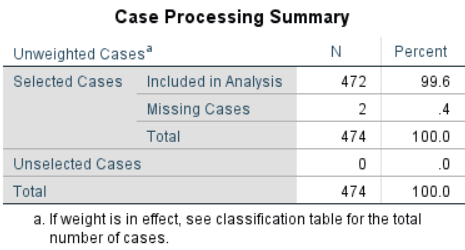
\includegraphics[width=0.8\textwidth]{images/501.PNG}
\end{figure}

\vspace{1.5cm}
Από τον πίνακα \textbf{\lat{Case Processing Summary}} παρατηρούμε ότι για την εξαρτημένη μεταβλητή υπάρχουν 2 \lat{missing cases}.

Στον πίνακα \lat{Dependent Variable Encoding} φαίνεται η εσωτερική κωδικοποίηση της εξαρτημένης μεταβλητής και στον πίνακα \lat{Categorical Variables Codings} φαίνεται η κωδικοποίηση της κατηγορικής ανεξάρτητης μεταβλητής. 

\clearpage

\begin{figure}[h]
    \centering
    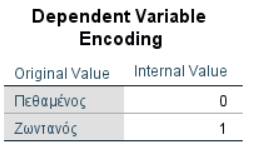
\includegraphics[width=0.4\textwidth]{images/502.PNG}
\end{figure}

\vspace{0.5cm}
\begin{figure}[h]
    \centering
    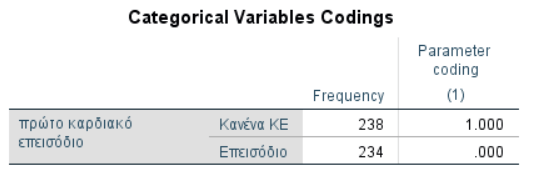
\includegraphics[width=0.6\textwidth]{images/503.PNG}
\end{figure}

Ο πίνακας \lat{Classification Table} περιέχει μόνο το σταθερό όρο. Όλες οι τιμές της εξαρτημένης μεταβλητής κατατάσσονται στην κατηγορία με τη μεγαλύτερη συχνότητα , δηλαδή στην υποκατηγορία “Ζωντανός”.

\begin{figure}[h]
    \centering
    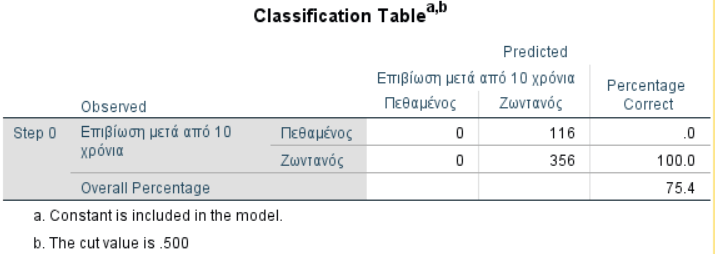
\includegraphics[width=0.8\textwidth]{images/504.PNG}
\end{figure}

\vspace{1cm}
Ο πίνακας \textbf{\lat{Variables in the Equation}} μας δίνει πληροφορίες μόνο για το σταθερό όρο. 

Ο πίνακας \textbf{\lat{Variables not in the Equation}} μας δίνει πληροφορίες για την αξιολόγηση των ανεξάρτητων μεταβλητών που δεν έχουν εισέλθει ακόμη στο υπόδειγμα. Δηλαδή εξετάζει τη σημαντικότητα κάθε μιας από τις ανεξάρτητες μεταβλητές εάν έμπαινε μόνη της στο υπόδειγμα μαζί με το σταθερό όρο. Το κριτήριο είναι το \textbf{\lat{Score}} το οποίο μας δείχνει ποια μεταβλητή έχει μεγαλύτερη βαρύτητα στην πρόγνωση της εξαρτημένης μεταβλητής. Στη δική μας περίπτωση μεγαλύτερη βαρύτητα φαίνεται να έχει η μεταβλητή Πρώτο καρδιακό επεισόδιο.   

\clearpage

\begin{figure}[h]
    \centering
    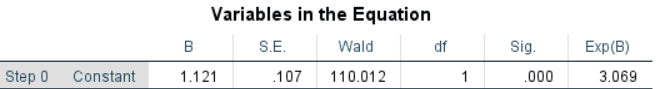
\includegraphics[width=0.8\textwidth]{images/505.PNG}
\end{figure}

\begin{figure}[h]
    \centering
    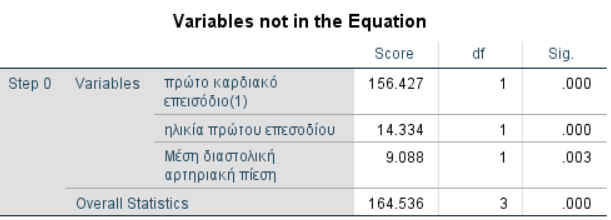
\includegraphics[width=0.8\textwidth]{images/506.PNG}
\end{figure}

\vspace{1cm}
Ο πίνακας \textbf{\lat{Omnibus Tests of Model Coefficients}} περιλαμβάνει τις τιμές για τα p-value οι οποίες μας δείχνουν το επίπεδο στατιστικής σημαντικότητας. Παρατηρούμε ότι p < 0,05 επομένως οι ανεξάρτητες μεταβλητές συνδυαζόμενες μεταξύ τους συμβάλλουν σημαντικά στην πρόγνωση των τιμών της εξαρτημένης. 
\vspace{1cm}

\begin{figure}[h]
    \centering
    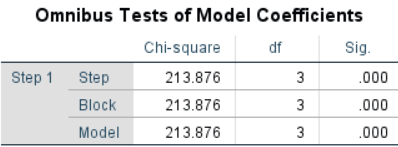
\includegraphics[width=0.8\textwidth]{images/507.PNG}
\end{figure}

\vspace{1cm}
Στον πίνακα Model Summary δίνεται η τιμή της συνάρτησης λογαριθμο-πιθανοφάνειας μαζί με το συντελεστή προσδιορισμού Cox \& Snell και το συντελεστή Nagelkerke. Από αυτούς τους συντελεστές φαίνεται ότι η μεταβλητότητα της εξαρτημένης μεταβλητής ερμηνεύεται από τις τρεις ανεξάρτητες μεταβλητές του λογαριθμικού υποδείγματος σε ποσοστό 36\% – 54\%. 

\clearpage

\begin{figure}[ht]
    \centering
    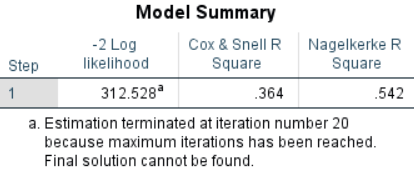
\includegraphics[width=0.8\textwidth]{images/508.PNG}
\end{figure}
\vspace{1cm}
Ο έλεγχος Hosmer and Lemeshow έχει ως υποθέσεις τις εξής:
\begin{itemize}
    \item \lat{$H_0$} : Το μοντέλο έχει καλή προσαρμογή 
    \item \lat{$H_1$} : Το μοντέλο δεν έχει καλή προσαρμογή 
\end{itemize}

Από τον πίνακα παρατηρούμε πως το p – value είναι μεγαλύτερο από 0,05 επομένως το μοντέλο μας προσαρμόζεται ικανοποιητικά στα δεδομένα.
\vspace{1cm}

\begin{figure}[h]
    \centering
    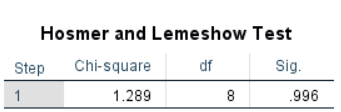
\includegraphics[width=0.6\textwidth]{images/509.PNG}
\end{figure}

\vspace{1cm}
Ο πίνακας ταξινόμησης \lat{Classification Table} δείχνει το ποσοστό στο οποίο συμφωνούν οι παρατηρούμενες και οι εκτιμώμενες από το υπόδειγμα τιμές της εξαρτημένης μεταβλητής. Στην περίπτωσή μας το ποσοστό αυτό ανέρχεται σε 78,4\%.

\clearpage

\begin{figure}[ht]
    \centering
    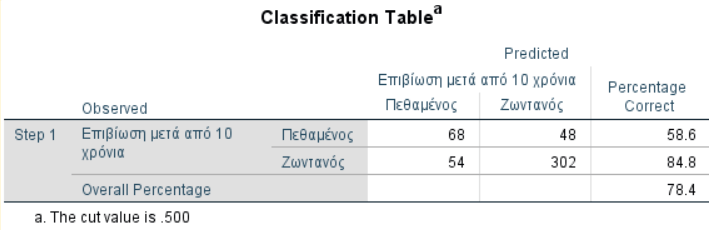
\includegraphics[width=0.8\textwidth]{images/510.PNG}
\end{figure}

Ο πίνακας Variables in the Equation μας δείχνει τους συντελεστές του υποδείγματος μαζί με τους αντίστοιχους επαγωγικούς ελέγχους και τα διαστήματα εμπιστοσύνης τους . 
\vspace{1cm}

\begin{itemize}
    \item Η στήλη Β αναγράφει τις τιμές των συντελεστών των ανεξάρτητων μεταβλητών που συνδέονται στατιστικά σημαντικά με την εξαρτημένη.
    \item Η στήλη \lat{S.E.} δείχνει το τυπικό σφάλμα της εκτίμησης της τιμής του κάθε συντελεστή.
    \item Το κριτήριο \lat{Wald} μας δείχνει κατά πόσο είναι σημαντική η επίδραση των ανεξάρτητων μεταβλητών στη διαμόρφωση των τιμών της εξαρτημένης. 
    \item Η στήλη \lat{Sig.} αποδεικνύει τη στατιστική σημαντικότητα των μεταβλητών που συμμετέχουν στο μοντέλο της παλινδρόμησης.
    \item Οι δύο τελευταίες στήλες του πίνακα μας δίνουν τα όρια ενός 95\% διαστήματος εμπιστοσύνης για τον κάθε ένα συντελεστή των ανεξάρτητων μεταβλητών.
\end{itemize}

\vspace{1cm}

\begin{figure}[h]
    \centering
    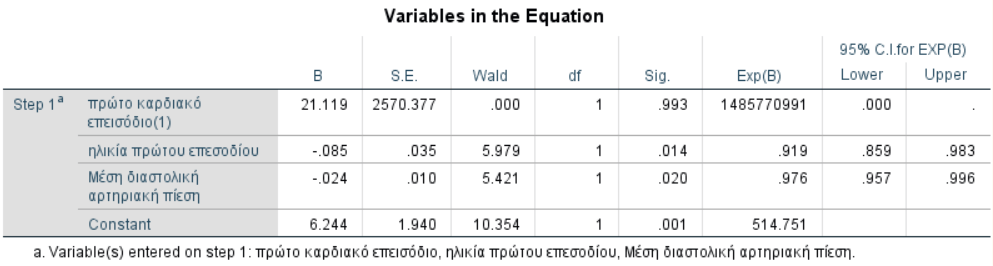
\includegraphics[width=\textwidth]{images/511.PNG}
\end{figure}

\clearpage
Ολοκληρώνοντας το λογαριθμικό μας μοντέλο καταλήξαμε στα εξής συμπεράσματα:

\begin{itemize}
    \item Πριν εισαχθούν οι ανεξάρτητες μεταβλητές στο λογαριθμικό μοντέλο η μεταβλητή με τη μεγαλύτερη βαρύτητα στην πρόγνωση της εξαρτημένης μεταβλητής είναι το Πρώτο καρδιακό επεισόδιο (\lat{Score} $=$ 156,427) . Ύστερα όμως από την εισαγωγή τους στο μοντέλο , παρατηρούμε ότι το πρώτο καρδιακό επεισόδιο δεν επιδρά σημαντικά στη διαμόρφωση τιμών της εξαρτημένης μεταβλητής (\lat{Wald} $=$ 0,000) και αυτό φαίνεται επίσης από το γεγονός ότι το p – value είναι μεγαλύτερο από 0,05  .
    \item Παρ’ όλα αυτά επιλέξαμε μία από τις ανεξάρτητες μεταβλητές μας να είναι το πρώτο καρδιακό επεισόδιο , διότι κάνοντας επιπλέον συνδυασμούς απουσίας της συγκεκριμένης ανεξάρτητης μεταβλητής , το λογαριθμικό μοντέλο δεν προσαρμοζόταν καθόλου ικανοποιητικά στα δεδομένα μας .
    \item Με βάση τον τελευταίο πίνακα το υπόδειγμα έχει τη μορφή : 
  
    \vspace{1cm}
    
    (Πιθανότητα επιβίωσης μετά από 10 χρόνια) $=$ 6,244$+$21,119 (πρώτο καρδιακό) $-$ 0,024 (δαπ) $-$ 0,085 (ηλικία πρώτου επεισοδίου)  
    
\end{itemize}